\section{Aufbau}
Der Aufbau wird aufgeteilt in drei verschiedene Elemente. Zum einen die Quelle, wobei hier $^{137}\text{Cs}$ verwendet wurde, 
zum anderen das zu durchleuchtende Objekt und letzlich den Detektoraufbau. 
Die Quelle selbst wird aus Strahlenschutzgründen von Blei umgeben wobei eine kleine Öffnung dem Strahl erlaubt zum Detekor zu gelangen.
Als Target werden in dem Versuch mehrere Würfel gewählt, mit der Dimension von $\SI{3}{\centi\meter}$ x $\SI{3}{\centi\meter}$ x $\SI{3}{\centi\meter}$,
wobei diese im Inneren weitere Elemantarwürfel enthalten. Disese sind ebenfalls quadratisch mit einer Seitenlänge von $\SI{1}{\centi\meter}$.
Es passen also in einen 27 kleinere Elemantarwürfel mit symmetrischer Anordnung. Umgeben ist das Ensemble von Elemantarwürfeln, i. e.
der große Würfel, von einer $\SI{1}{\milli\meter}$ dicken Schicht aus Alluminium. Diese Hülle bietet zusätzlichen Platz um 
den Targets eine Nummer zuzuweisen. So hat der Würfel mit der $1$ keine inneliegenden Elemantarwürfel, folglich also besteht er nur aus
der Alluminiumummantelung. Anders sind die Würfel 2 und 3, welche vollständig mit 27 Elemantarwürfeln gefüllt sind.
Jeder Elementarwüfel, in einem größeren Würfel, besteht aus dem gleichen Material. Die Menge an möglichen Elementen die für die Absorption 
interessant sind sind also: Alluminium, $\text{Material}_{1}$, $\text{Material}_{2}$.
Ein letzter Würfel trägt die Nummer 4 und ist mit Elemantarwürfeln verschiedener Materialen, jedoch solcher, die auch in den Würfeln 1 und 2 vertreten sind, gefüllt.
Jeder dieser Targets kann auf eine Montur direkt in den Strahlengang gelegt -und auf dieser verschoben und rotiert werden.
\\
\newline
Die abgeschwächte $\gamma$-Strahlung wird letztlich in einen Detekor geleitet, der maßgeblich aus einem anorganischen NaJ-Szinitillator besteht.
Dieser lässt Ionisationen durch \enquote{Lichtblitze} messbar werden, wobei die Intensität solcher deutlich zu schwach für weitere Schritte ist.
Ein Photomultiplier verstärkt durch Dynoden die einfallenden Lichtblitze und liefert so eine verwendbare Größe, durch einen Diskriminator, 
an einen Multichannelanalyzer. Der Diskriminator hindert ungewollte Störsignale durch den Szinitillator zu passieren und liefert so genauere Messungen.
Die graphische Auswertung erfolgt in Echtzeit an einem , der mit dem Multichannelanalyzer verbunden ist. Hier werden die Signale 
der Energie nach einem \enquote{Channel} zugewiesen und jeder weitere Einfall mit genau gleicher Energie als \enquote{Count} dem Kanal hinzugefügt.

\section{Durchführung}
Zu Beginn wird Aufschluss über die Absorptionskoeffizienten der drei Materialen gewonnen. 
Dafür werden die Würfel 1 bis 3 auf der Montur in den Strahlengang gelegt, sodass, sollten Elemantarwürfel enthalten sein, jeweils eine Zeile solcher elementaren Würfel 
durchstrahlt wird. Das Programm  \enquote{MAESTRO} am PC wird gestartet und misst für $\SI{300}{\second}$ die einfallende Strahlung am Detekor. Drei Messreihen pro Würfel, also jede Zeile einmal, geben genug Aufschluss über den anschließend gemittelten Absorptionskoeffizienten.
Final wird der Würfel mit Nummer 4 durchleuchtet. Hier ist das Material nicht homogen, es kommt also stark auf die Ausrichtung zum Strahl an, welche Stärke
die Abschwäschung hat. Es folgen 12 Messungen, beginnend mit dem Abfahren der drei Zeilen wie davor auch. Anschließend wird der Würfel um 
$\frac{\pi}{4}$ wahlweise nach links oder rechts gedreht, wobei die Richtung bei der Auswertung sehrwohl eine Rolle spielt.
Nun soll der Strahlengang genau so ausgreichtet werden, dass eben zwei dann drei und wieder zwei unterschiedliche Elementarwüfel bei gleichbleibender Drehung
durchleuchtet werden. Nach erneuter Rotation um $\frac{\pi}{4}$ in die gleiche Richtung wiederholt sich der Schritt um 
allen 12 Messreihen nachzukommen.

\section{Messwerte}
Für die Auswertung von Bedeutung ist nicht das komplette Spektrum der Strahlung, sondern es genügt sich die maximal auftretende Energie mit enstprechendem
Channel über den Versuch hinweg anzuschauen. Bei etwaiger Absorption durch Würfel im Strahlengang darf sich so die Verteilung nicht verschieben, sondern 
nur die Amplitude, die hier durch Counts dargestellt ist, verringern.
Um Festzustellen welcher Channal sich eignet wird eine Messreihe ohne Würfel gestartet, wobei ein deutliches Maximum an Counts bei dem Kanal 157 gefunden wurde. Dieser Peak der \ce{^{137}_{}Cs}-Quelle lässt sich dem typischen Energiewert
$E = \SI{661.7}{\kilo\electronvolt}$ zuordnen.


\begin{figure}
    \centering
    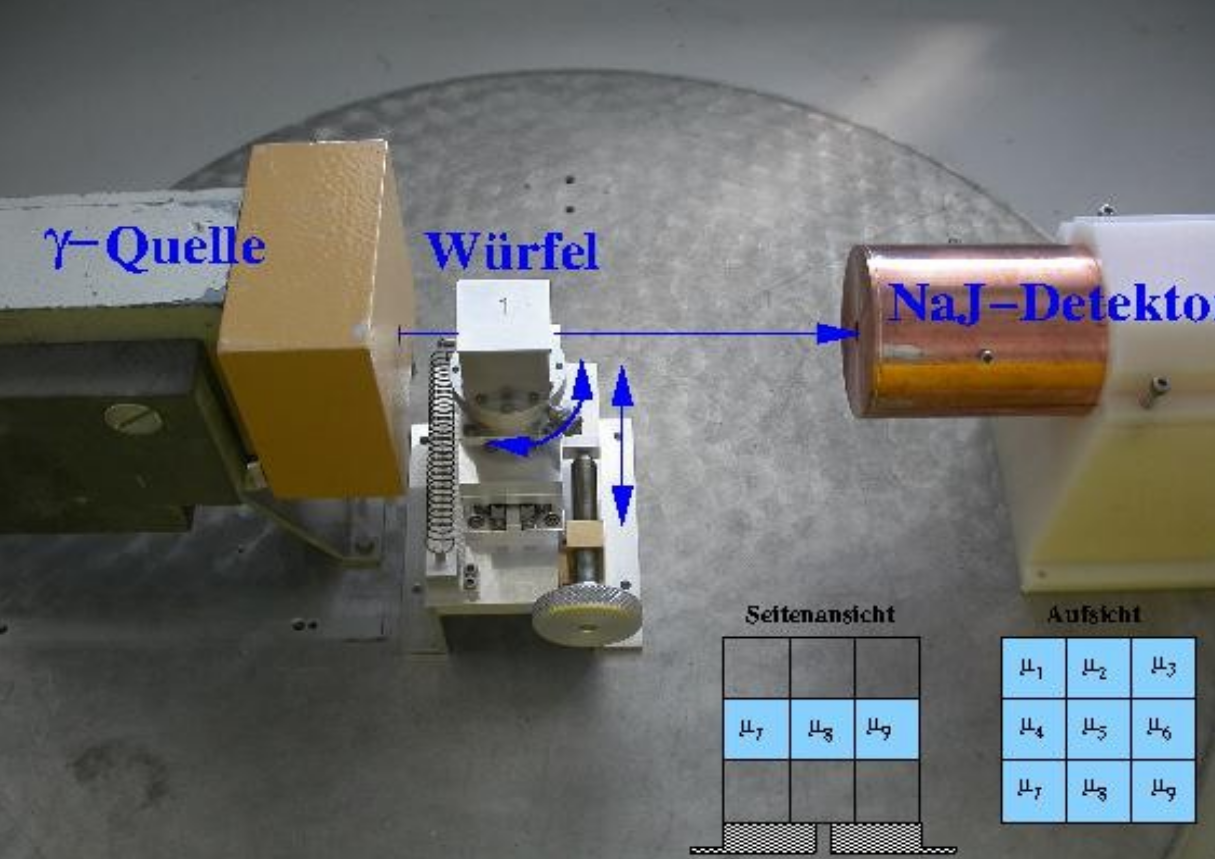
\includegraphics[width=0.9\textwidth]{bilder/test.png}
    \caption{Die Abbildung zeigt einen Aufbau um durch Tomographie Aufschluss über den Inhalt eines Würfels, gefüllt mit Elementarwürfeln zu bekommen.
    Links im Bild strahlt eine bleiverdeckte Quelle auf den zentrierten Würfel. Rechts im Bild ist ein Detekor zu sehen. \cite{skript}}
    \label{fig:1}
\end{figure}
